\documentclass[journal,twoside,web]{ieeecolor}
\usepackage{generic}
\usepackage{cite}
\usepackage{amsmath,amssymb,amsfonts}
\usepackage{algorithmic}
\usepackage{graphicx}
\usepackage{textcomp}
\def\BibTeX{{\rm B\kern-.05em{\sc i\kern-.025em b}\kern-.08em
    T\kern-.1667em\lower.7ex\hbox{E}\kern-.125emX}}
\markboth{Miguel Faggioni}
{Author \MakeLowercase{\textit{et al.}}: Sistemas de Control Multivariable - Miguel Faggioni}
\begin{document}
	
\title{Análisis de Sistemas de Control Multivariable (Caso de estudio)}
\maketitle

\begin{abstract}
En el presente trabajo se estara analizando una planta asociada a la industria manufacturera con el fin de poner a pruebas este sistema a distintos esquemas de control. Se analizara el sistema con esquemas de control centralizados y descentralizados.
\end{abstract}


\section{Descripción de la Planta}
En la producción de laminadoras de bandas en caliente, la calidad de las bandas es una de las más factores importantes para la satisfacción del consumidor. Por lo general se expresa en términos del espesor de la tira y el ancho de la misma. Dado que el proceso de laminación de bandas es parte del ultimo proceso que se debe completar para finalizar el producto es importante mantener altos niveles de calidad.

Es importante mantener una calidad de producción estable con un diseño de sistema de control en el proceso de laminación en caliente / frío. El proceso para ajustar el grosor de la tira esta principalmente controlado por un subsistema de válvulas, que a su vez controla un sistema de rodillos. Este proceso AGC esta modelado en general por la  ecuación del resorte

\begin{equation}
	h = S + \frac{P}{C}
\end{equation}

donde $C$ es la rigidez equivalente del soporte del molino, $h$ grosor de la lamina, $P$ la fuerza de rodadura y $S$ la brecha de los rodillos. La diferencia de espacio entre rodillos $\Delta S$es el parámetro clave a ser controlado por el sistema AGC, que conducirá a la cambio en la fuerza de rodadura $\Delta P$ basada en la ecuación del resorte. Esto da como resultado la fluctuación de los parámetros del rodillo horizontal de flexión y de deformación de corte, que a su vez causa desviaciones en la corona de la tira. Por otro lado en el sistema de control de la corona, el parámetro clave controlado es el cambio en las fuerzas de flexión $\Delta F$, que compensará de giro, pero puede conducir a la desviación de las fuerzas de los rodillos como una perturbación externa y luego causar un parámetro efecto de acoplamiento en el sistema AGC. Basado en lo anterior, el sistema de control de espesor de la corona se puede definir como un sistema multivariado típico con fuertes efectos de acoplamiento. Basado en investigaciones anteriores [2], [3] el sistema de control del grosor de la corona puede ser modelado por

\begin{equation}
	\begin{bmatrix}
		 \Delta h  \\
		 \Delta CR 
	\end{bmatrix} = G(s) \begin{bmatrix}
							 \Delta S  \\
							 \Delta F 
	  					\end{bmatrix}
\end{equation}


donde $\Delta CR$ es el cambio en el grosor de la corona y $\Delta h$ es el cambio en el espesor de la tira. Usando la teoría estándar de identificación de sistemas [4], el Parámetros del laminador de bandas en caliente para un punto de ajuste nominal. de 1700 mm y una velocidad de rodadura de 13 m/s puede ser determinada como [3]:

\begin{equation}
	\begin{bmatrix}
		 \Delta h  \\
		 \Delta CR 
	\end{bmatrix} = \begin{bmatrix}
			G_{11}(s) & G_{12}(s) \\
			G_{21}(s) & G_{22}(s)
	\end{bmatrix} \begin{bmatrix}
							 \Delta S  \\
							 \Delta F 
						\end{bmatrix}
\end{equation}

	\begin{equation}
		\begin{bmatrix}
		\Delta h  \\
		\Delta CR 
		\end{bmatrix} = \begin{bmatrix}
							\frac{0.00025s + 0.025}{0.00075s^2 + 0.065s + 1} & 	\frac{0.001}{0.0002s^2 + 0.03s + 1} \\
							\frac{0.00025s + 0.025}{0.00075s^2 + 0.065s + 1} & \frac{0.025}{0.0002s^2 + 0.03s + 1}
						\end{bmatrix} \begin{bmatrix}
											\Delta S  \\
											\Delta F 
										\end{bmatrix}
	\end{equation}

En la práctica, la velocidad de rodadura puede variar entre 10 y 16 m/s, Esto lleva al potencial de un cambio del 20\% en los parámetros. [2]. En términos generales, la incertidumbre puede ser cualquiera aditivo o multiplicativo. En el sistema de grosor de corona, La incertidumbre es multiplicativa, ya que se origina a partir de la velocidad de rodadura.


	\subsection{Modelo en Espacio de Estados}

Teniendo en cuenta que el sistema sera analizado por un sistema de control centralizado, debemos obtener el una realización en espacio de estados del caso de estudio. 
Para esto se uso las herramientas de conversión de sistemas SIMO que ofrece Matlab.

	\begin{equation}
		\begin{aligned}
			\begin{bmatrix}
				\dot{x_1}(t)  \\
				\dot{x_2}(t)  \\
				\dot{x_3}(t)  \\
				\dot{x_4}(t) 
			\end{bmatrix} = \begin{bmatrix}
								86.70 & -1333.30 & 0 & 0 \\
								1     & 0        & 0 & 0 \\
								0 & 0 & -150 & -5000 \\
								0 & 0 & 1 & 0 
							\end{bmatrix} \begin{bmatrix}
										x_1(t)  \\
										x_2(t)  \\
										x_3(t)  \\
										x_4(t) 
										\end{bmatrix} \\ + \begin{bmatrix}
												1 & 0 \\
												0 & 0 \\
												0 & 1 \\
												0 & 0
											\end{bmatrix}  + \begin{bmatrix}
																u_1(t) \\
																u_2(t)
															\end{bmatrix}
		\end{aligned}
	\end{equation}

	

\section{Análisis a Lazo Abierto del Sistema}

	\subsection{Estabilidad}
		
		Para este ítem se analizaran los auto-valores del sistema a lazo abierto teniendo en cuenta la representación en variables estados de la planta. De esta forma los mismos están localizados en la siguientes coordenadas del plano complejo
		
		\begin{equation}
			\begin{bmatrix}
				-66.67 \\
				-20.00 \\
				-100.00 \\
				-50.00
			\end{bmatrix}
		\end{equation}
		
		Los auto-valores están claramente localizados en el semi-plano izquierdo del plano complejo. Lo que permite concluir que el sistema es estable.
		
	\subsection{Análisis de Interacciones}
	
		En términos de interacciones se procedió al calculo del arreglo de ganancia relativa a fin de poder establecer los posibles emparejamientos entre las entradas y salidas del sistema.
		
		Para esto veamos la matriz $K$, asociada al sistema
		
		\begin{equation}
			K = \begin{bmatrix}
				0.025 & 0.001 \\
				0.025 & 0.025
			\end{bmatrix}
		\end{equation}
		
		Así
		
		\begin{equation}
		\label{rga}
			\varLambda = K .* {K^{-1}}^{T} = \begin{bmatrix}
												1.0417 & -0.0417 \\
												-0.0417 & 1.0417
											\end{bmatrix}
		\end{equation}
		
		Teniendo en cuenta el resulta anterior, es notable la influencia de la entrada 1 y 2 sobre las salidas 1 y 2 respectivamente. Esto permite establecer de forma clara los emparejamientos que permitirán establecer estrategias de diseño descentralizadas.
		
		
	\subsection{Respuesta al Escalón}
	
	Teniendo en cuenta el modelo matemático del sistema, se realizara en análisis del mismo en lazo abierto, para esto se realizaron simulaciones haciendo uso 
	del paquete de Simulación Simulink.
	
	\begin{figure}[h]
		\begin{center}
			\includegraphics[width=7cm,height=4cm,keepaspectratio]{modelsimulink}
			\caption{Modelo de Simulación a Lazo Abierto\label{modelsimulink}}
		\end{center}
	\end{figure}
	
	
	\begin{figure}[h]
		\begin{center}
			\includegraphics[width=8cm,height=4cm,keepaspectratio]{subsystemtf}
			\caption{Modelo de la planta \label{subsystemtf}}
		\end{center}
	\end{figure}	
	
	Al someter a la planta a entradas constantes se obtuvieron los resultados que se aprecian en la Figura \ref{olstepresponse}.
	
	\begin{figure}[h]
		\begin{center}
			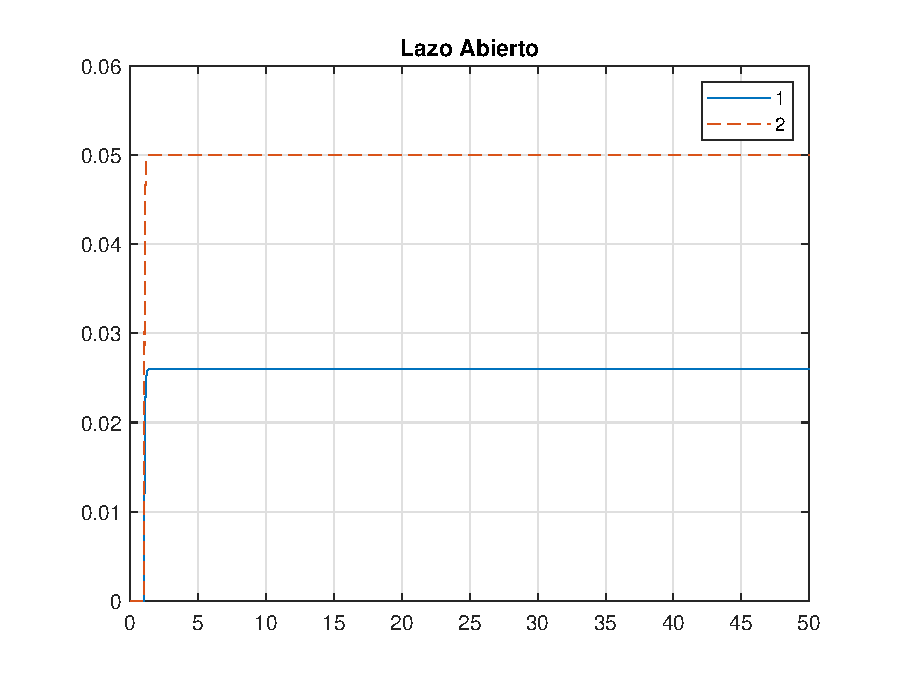
\includegraphics[width=6cm,height=6cm,keepaspectratio]{olstepresponse}
			\caption{ Respuesta del Sistema a lazo Abierto \label{olstepresponse}}
		\end{center}
	\end{figure}		
	
	De la gráfica podemos observar que el sistema de forma natural es estable, sin embargo, posee un problema importante en estado estable, es notable error de estado estacionario.


\section{Técnicas de Control Descentralizado}

	Una vez estudiado y analizado la planta bajo un esquema de control centralizado, procedamos a establecer una metodología descentralizada que permita obtener una buena respuesta del sistema. Para esto primero que nada, se tomo en cuenta el arreglo de ganancias relativas, tengamos en cuenta la ecuación \eqref{rga}. Así los apareamiento para implementar la estrategia de diseño son las siguiente:
	
	\begin{equation}
		\begin{aligned}
			u_1 \longrightarrow y_1 \\
			u_2 \longrightarrow y_2
		\end{aligned}
	\end{equation}
	
	El presente trabajo no tiene como objetivo ahondar en las diferentes técnicas de diseño de sistemas SISO, por lo que el uso de controlador PI en el presente trabajo se hizo de forma generalizada, así mismo, su sintonización fue realizada haciendo uso de técnicas clásicas. De esta manera, los controladores poseen la siguiente función de transferencia.
	
	\begin{equation}
		\begin{aligned}
			C_1(s) &= 81.85 + \frac{1000.50}{s} \\
			C_2(s) &= 5 + \frac{400}{s}
		\end{aligned}
	\end{equation}
	
	Tomando los controladores como punto de partida se realizo la siguiente simulación
	
	\begin{figure}[h]
		\begin{center}
			\includegraphics[width=6cm,height=6cm,keepaspectratio]{descentralizado}
			\caption{ Esquema de Control Descentralizado \label{descentralizado}}
		\end{center}
	\end{figure}
	
	\begin{figure}[h]
		\begin{center}
			\includegraphics[width=6cm,height=6cm,keepaspectratio]{clresponse}
			\caption{ Respuesta al Escalón  \label{clresponse}}
		\end{center}
	\end{figure}

	Es notable que se mejoro de gran forma el estado estacionario del  sistema.
	
	
	
	\newpage
\section{Técnicas de Control Centralizado}

	Para el esquema de control centralizado se establece el siguiente diagrama de bloques.


	\begin{figure}[h]
		\begin{center}
			\includegraphics[width=6cm,height=6cm,keepaspectratio]{sssystem}
			\caption{ Sistema de Control Centralizado \label{sssystem}}
		\end{center}
	\end{figure}

	Donde los subsistemas quedan expuesto a continuación
	
	
	\begin{figure}[h]
		\begin{center}
			\includegraphics[width=6cm,height=6cm,keepaspectratio]{centralizadosistema}
			\caption{ Sistema en Espacio de Estados \label{centralizadosistema}}
		\end{center}
	\end{figure}
	
	\begin{figure}[h]
		\begin{center}
			\includegraphics[width=6cm,height=6cm,keepaspectratio]{observer}
			\caption{ Sistema Observador \label{observer}}
		\end{center}
	\end{figure}
	
	Para este sistema se diseñaron matrices de ganancias tanto del controlador como del observador de la siguiente forma
	
	\begin{equation}
		K = \begin{bmatrix}
				-67.70 & -1273.30 & 0 & 0 \\
				0 & 0 & -131 & -4940
		\end{bmatrix}
	\end{equation}
	
	\begin{equation}
		L = \begin{bmatrix}
			509.54 & -20.38 \\
			-7.45 & 0.298 \\
			118.74 & 132.26 \\
			-1.36 & -1.13
		\end{bmatrix}
	\end{equation}

	\begin{figure}[h]
		\begin{center}
			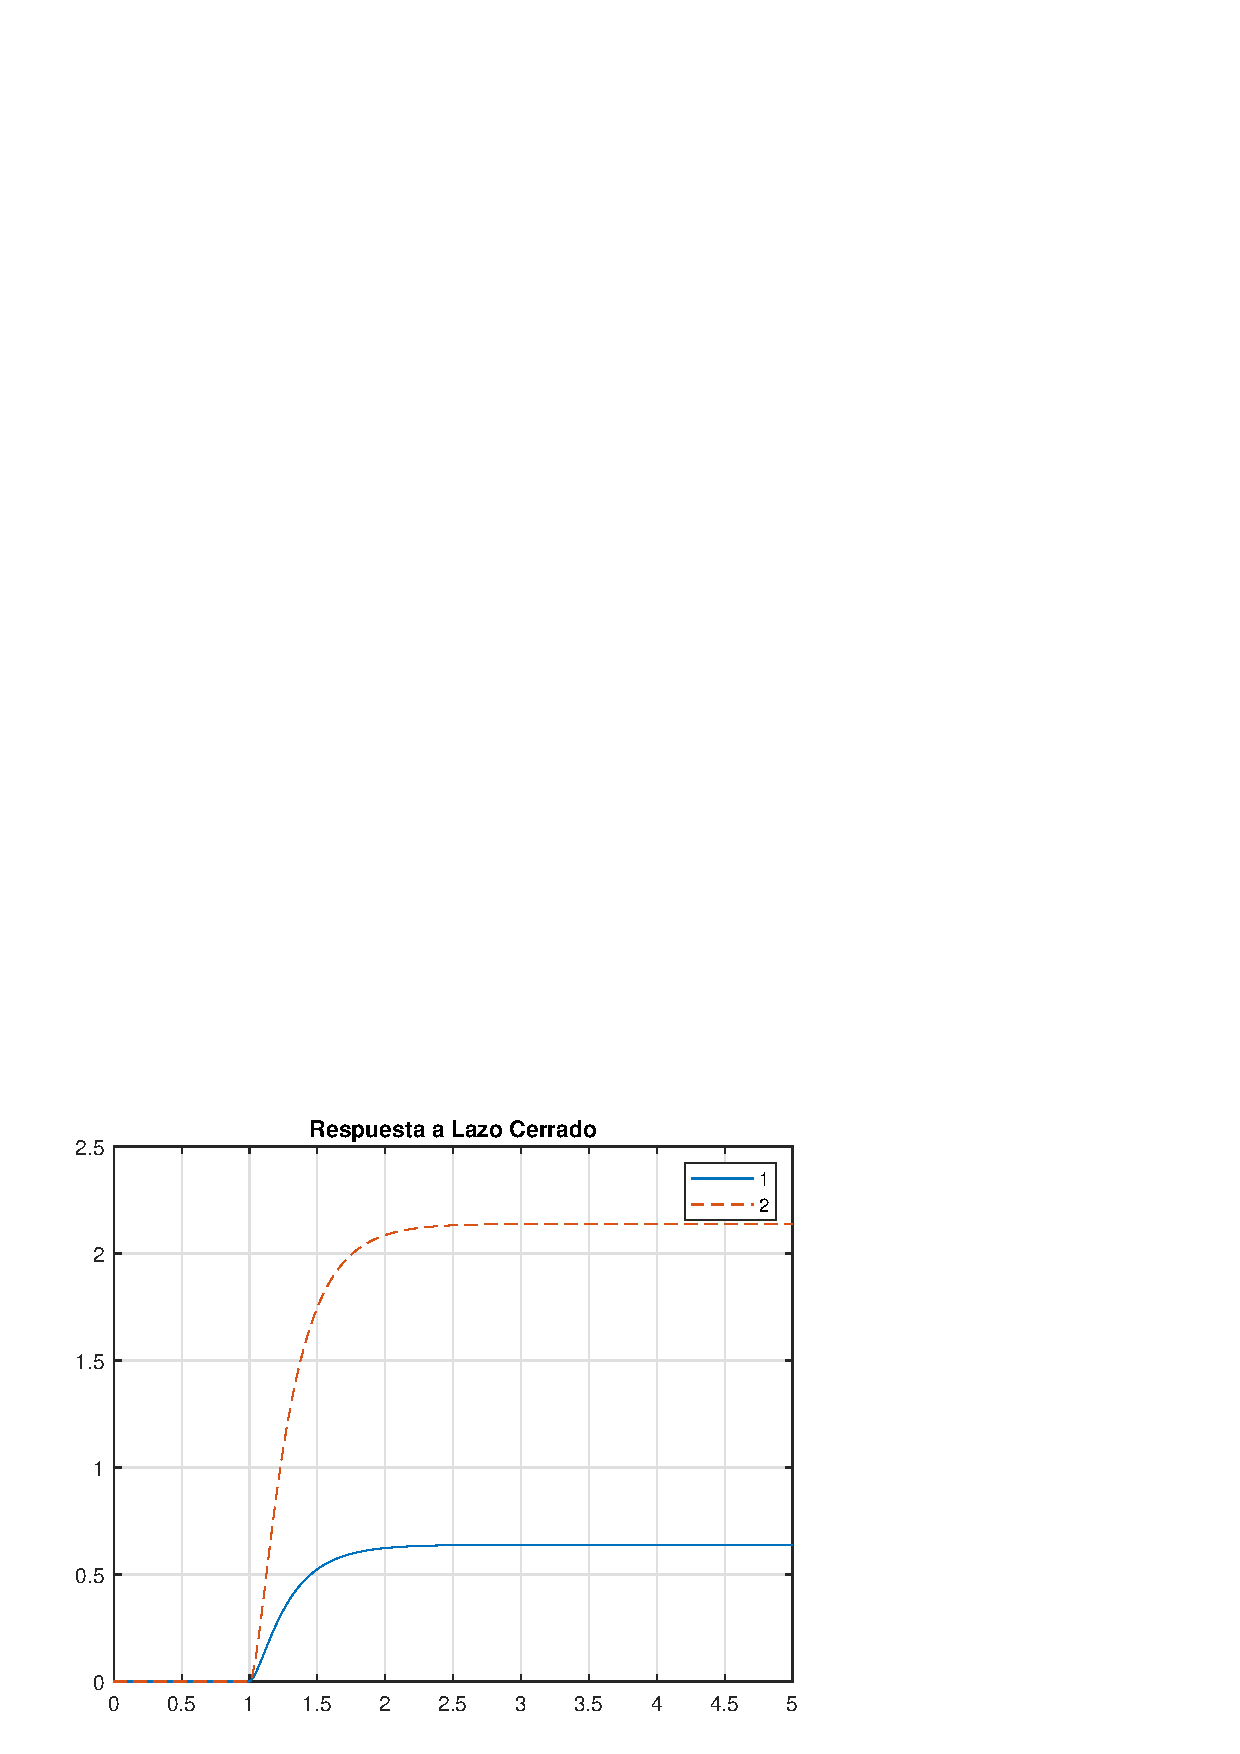
\includegraphics[width=6cm,height=6cm,keepaspectratio]{ssresposen}
			\caption{ Sistema Observador \label{ssresposen}}
		\end{center}
	\end{figure}

\section{Red de Desacople}

Al realizar el calculo del arreglo de ganancia relativa se determino que existe un sistema naturalmente desacoplado. De esta manera no hubo necesidad de establecer una red de desacople para este sistema de estudio.
	


	
\section{Conclusión}

Teniendo en cuenta los resultados expuesto se aprecia que las metodologías multilazo ofrecen una gran herramienta de control en sistemas multivariables. Permitir que el diseño de controladores caiga en el dominio de sistema SISO, ofrece una facilidad de implementación y diseño que los sistemas centralizados carecen notablemente. 

Así mismo, el arreglo de ganancia relativa resulta ser una herramienta que de manera sencilla permite establecer sin recurrir a demasiado calculo el enfoque desde el punto de vista de control que se debe implementar.	


\begin{thebibliography}{00}

\bibitem{b1} Kersting, S ``Direct and Inndirect Model Reference Adaptative Control for Multivariable Piecewise Affine Systems,'' IEEE Trans. Automat. Control, vol. 62, No. 11, pag 5634 - 5649 Nov. 2017.

\bibitem{b2} Y. Sun,  ``The Model and Control of Cold and Hot Strip Mill,'' Beijing, China: Metallurgical Industry Press, 2010.

\bibitem{b3} P. Jing, and C. Tonng,  ``Decoupling based robust control strategy for shape and gauge system,'' Inf. Control, vol. 40. no. 4, pp. 467-471, 2011.

\bibitem{b4} Y. A. W. Shardt,  ``Statistics for Chemical and Proccess Engineers: A modern Approach,'' . Switzerland: Springer, 2015.

\end{document}
